\section*{Results}

\begin{table}[htbp]

\begin{tabular}{lllll}
\toprule
{} & samples (RNA) &         Mutations &   Neoantigens & Expressed Neoantigens \\
\midrule
ascites pre-treatment                 &         4 (4) &  10148 $\pm$ 1000 &  199 $\pm$ 60 &           78 $\pm$ 30 \\
ascites post-treatment                &       24 (20) &  13428 $\pm$ 1000 &  295 $\pm$ 50 &          143 $\pm$ 30 \\
\textit{model adjusted change (\%)} &               &       57 $\pm$ 65 &   65 $\pm$ 94 &         117 $\pm$ 142 \\
\hline
solid pre-treatment                   &       76 (70) &    7806 $\pm$ 900 &  152 $\pm$ 20 &            63 $\pm$ 9 \\
solid post-treatment                  &        11 (4) &  11079 $\pm$ 3000 &  264 $\pm$ 90 &           38 $\pm$ 20 \\
\textit{model adjusted change (\%)}   &               &        6 $\pm$ 28 &   11 $\pm$ 41 &          -43 $\pm$ 35 \\
\bottomrule
\end{tabular}

\caption{\textbf{Mean mutations, neoantigens, and expressed noeantigens by sample type and chemotherapy treatment status.} The model-adjusted change is calculated using a Bayesian model that controls for technical variables affecting mutation identification, but does not separate treatment from coincident effects such as surgery and drift. Model effects and means are shown with 95\% credible regions and bootstrapped errors of the mean, respectively.}
\label{tab:cohort}
\end{table}

\begin{figure}[htbp]
\centering
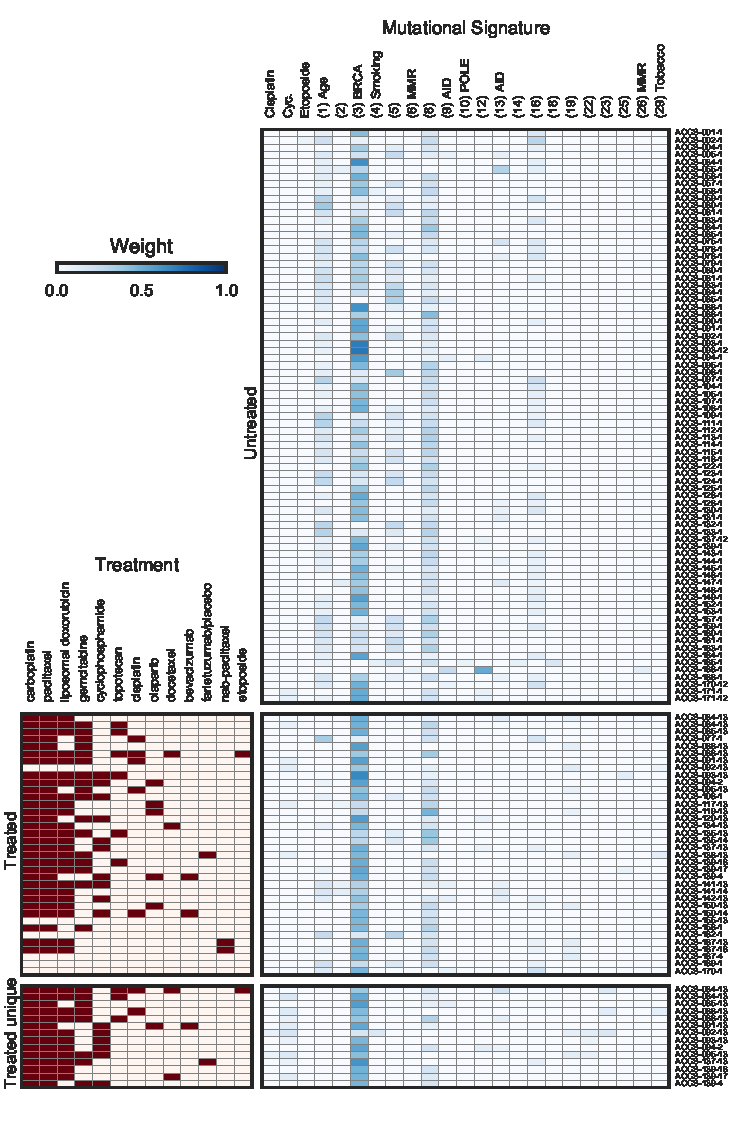
\includegraphics[scale=1.0]{figures/signatures.pdf}
\caption{\textbf{Treatments and detected mutational signatures for paired pre-/post-chemotherapy samples.} \textit{(Top)} Signatures detected in the pre-treatment samples. The first five signatures were extracted from reports of a \textit{G. gallus} cell line and \textit{C. Elegans} organisms after exposure to chemotherapy. The remaining signatures are from the COSMIC signature resource and give the COSMIC signature number in parentheses. \textit{(Bottom)} Clinical treatments and detected signatures for the mutations unique to the post-treatment samples. Cases where a chemotherapy signature is detected are annotated by level of agreement with the clinical record. A (*) indicates the donor received the drug (grouping cisplatin and carboplatin together), and a (?) indicates no record of the donor receiving the drug. Signatures not shown were undetected in these samples.}
\label{fig:signatures}
\end{figure}

\begin{figure}[htbp]
\centering
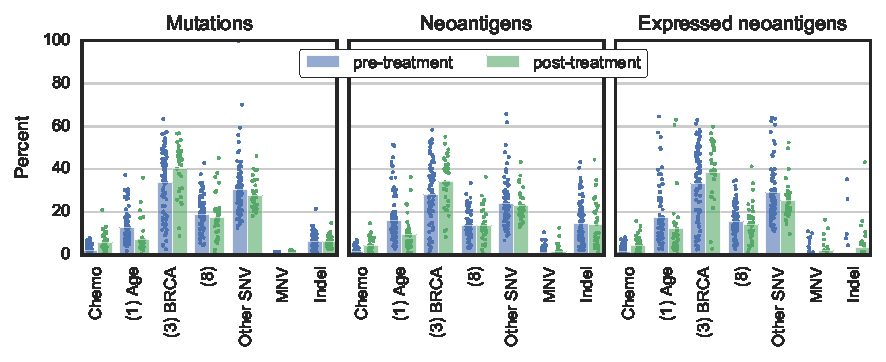
\includegraphics[scale=1.0]{figures/sources_of_mutations_and_neoantigens.pdf}
\caption{\textbf{Sources of mutations and neoantigens:} the estimated fraction of mutations \textit{(left)} and neoantigens \textit{(right)} generated by SNVs from various signatures, multinucleotide variants (MNVs), and indels. The \textit{Chemo} category combines the SNV signatures extracted from the \textit{G. gallus} and \textit{C. Elegans} studies. COSMIC signature numbers are in parentheses. The \textit{Other} category shows SNVs from COSMIC signatures other than the ones shown. The \textit{Unclassified} category shows SNVs that were not accounted for by the signature deconvolution (unknown signatures or a mix of processes). Error bars give the 95\% error of the mean by bootstrapping on samples.}
\label{fig:sources}
\end{figure}

% The treated samples showed more mutations, neoantigens, and, in the case of ascites samples, more expressed neoantigens (Table~\ref{tab:cohort}).

% STATEMENT_TREATMENT_EFFECT 
For 11/12 donors with paired pre- and post-treatment samples, somatic mutation burden increased after treatment (Figure~\ref{fig:supp_paired}). We developed a Bayesian model to estimate the magnitude of this increase using paired and unpaired samples and controlling for sample type and purity. The model estimated that treated samples have 57\% more mutations than untreated with 95\% confidence that the increase is at least 5\% (Figure~\ref{fig:bayesian_model_effects}).

%found with 95\% certainty that mutational burden increases by at least 5\% with treatment; mean effect was a 57\% increase.

% 95\% posterior probability 95\% posterior probability, this model confirmed that the number of mutations increases by at least 5\% with treatment, with a point estimate of 57\%.

% that the post-treatment timepoint is associated with at least a 5\% increase in mutations, and the mean effect size was 57\%.

% mutations increasing by at least 5\% with treatment; the  the estimated the effect of treatment to be a 57\% increase in mutations (Figure~\ref{fig:bayesian_model_effects}) and with there was a 95\% probability that the increase with treatment was as least 5\%.

% (95\% credible region 0--131)

% STATEMENT_NEOANTIGENS1
Using sequence-based HLA typing and computational pMHC binding prediction, across the cohort we identified 18,336 mutated peptides predicted to bind autologous MHC class I with affinity $\leq 500$nm, which we refer to as neoantigens. All but 26 (0.14\%) neoantigens were private to a single donor. Neoantigens tracked the increase in mutational burden after chemotherapy. In the Bayesian analysis, treated samples had 65\% (-14--174) more neoantigens, and, for ascites samples, 117\% (3--286) more expressed neoantigens. Interestingly, solid tumor samples showed an increase in neoantigens but a 43\% (2--71) decrease in expressed neoantigens.

Signature deconvolution was performed separately on all samples onto the 30 mutational signatures curated by COSMIC\cite{364242}, plus four additional signatures extracted from a study of cisplatin-exposed \textit{C. Elegans}\cite{Meier_2014}, and a chicken cell line exposed to cisplatin, cyclophosphamide, and etoposide\cite{Szikriszt_2016}. The top signatures were COSMIC \textit{Signature 3}, associated with BRCA disruption, \textit{Signature 8}, of unknown etiology, and \textit{Signature 1}, associated with a slow mutagenic process active in normal tissue. These signatures together accounted for over half of the mutations and neoantigens in both treated and untreated samples.

The etoposide and \textit{C.Elegans} and \textit{polq-1} knockout cisplatin signatures were found in nine and three of the 80 primary samples, 

The cyclophosphamide, etoposide,  

The \textit{G. gallus} cyclophosphamide signature was detected in 4/80 pre-treatment samples and 9/35 post-treatment samples, three of whom had a clinical record of cyclophosphamide treatment. This signature may have some association with cyclophosphamide treatment but appears to have a very high false-positive rate. The \textit{G. gallus} etoposide signature was detected in more pre-treatment samples than post-treatment, indicating it has no utility as marker of treatment. The \textit{C. Elegans} cisplatin signature from wildtype worms was not detected in any samples, but the signatures from three genetic knockouts were detected. The \textit{fcd-2} and \textit{xpf-1} knockout signatures each occurred in one cisplatin treated sample and no other samples. The \textit{polq-1} knockout signature seems less useful as marker, appearing in three untreated samples and four carboplatin-treated samples.

 the dominant signatures were largely the same in pre- and post-treatment samples (Figure and~\ref{fig:supp_signatures}). In both groups, the top signatures were 

For better sensitivity to detect chemotherapy-associated signatures, we next focused on the 14 samples from 12 donors with paired pre- and post-treatment samples. For each donor, we extracted the mutations that had evidence exclusively in the treated samples, requiring at least 30 reads coverage and zero variant reads in the pre-treatment samples. Of 229,132 SNV mutations in the post-treatment samples for these donors, we identified 106,171 such ``unique to treated'' mutations, over which we performed signature deconvolution (Figure ~\ref{fig:signatures}).

The \textit{G. gallus} cisplatin signature, previously undetected in all samples, was found in, and only in, the two cisplatin-treated samples available to this analysis, highlighting its potential utility as a marker of cisplatin (but not carboplatin) exposure. The \textit{C. Elegans} \textit{fcd-2} knockout was detected in three samples, all having received carboplatin but not cisplatin. COSMIC signatures \textit{3} and \textit{8} were detected in 14/14 and 9/14 post-treatment samples, respectively, but \textit{Signature 1} was completely absent, consistent with its association with slow mutagenic processes mostly at work before oncogenesis.

Within the paired samples and considering all chemotherapy-associated signatures except etoposide, at least one chemo signature was detected in 9/14 treated samples and 0/13 untreated samples. The magnitude of the effect of chemo-induced mutagenesis appears typically to be small, however, accounting for less than 12\% of the mutations or neoantigens in 13/14 samples (Figure~\ref{fig:sources}). The exception is sample AOCS-092-13, for which chemo signatures account for 24\% of the mutations and 18\% of the neoantigens. This donor is the most heavily treated in the cohort, having received eight distinct chemotherapeutic agents.
